\documentclass[../main/main.tex]{subfiles}

\newdate{date}{8}{11}{2019}


\begin{document}

\section{Zipper model}
\marginpar{ \textbf{Lecture 9.} \\  \displaydate{date}. \\ Compiled:  \today.}

The Zipper model is an unusually simple and interesting member of the class of one dimensional systems which exhibit a phase transition.
It is a model introduced by Kittel \cite{9_lesson_5} to describe oligomers undergoing \emph{denaturation transition}.
 Simplest model of DNA thermal denaturation transition (no bubbles). Better model for the denaturation of short oligomers.
 
The hypothesis are: the binding energy between two bases located at the end of the molecule is smaller than the one for pairs away from the ends. The unbinding starts and develops from the ends as a \emph{zipper}.
\begin{figure}[h!]
\centering
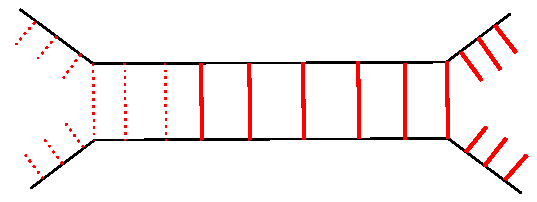
\includegraphics[width=0.6\textwidth]{../lessons/9_image/1.pdf}
\caption{\label{fig:9_1} Sequential unzipping from the ends.}
\end{figure}

\begin{figure}[h!]
\centering
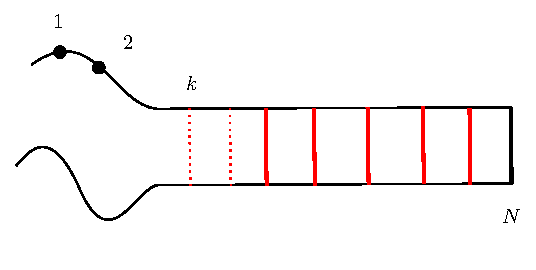
\includegraphics[width=0.6\textwidth]{../lessons/9_image/2.pdf}
\caption{\label{fig:9_2} Open and closed links in a single-ended zipper.}
\end{figure}

In this denaturation transition we do not allow bubbles.
Let us consider first the single-ended zipper, i.e. a molecular zipper of \emph{N} parallel links that can be opened only from one end as in Figure \ref{fig:9_2}. The single-ended zipper is simpler than any related problem which has been treated, and it offers a good way to introduce a biophysics example into a course of statistical mechanics.

If the first \emph{k} bonds (or links) are open (unbounded pairs) the energy to open the \emph{k+1} is \( \varepsilon _0 \). Note that if at least one of the previous \emph{k} bond is closed the energy needed to open the \( k+1 \) band is infinite! 
We specify further that the last link, \(k=N\), cannot be opened; this minor features serves only to distinguish one end from the other, and we shall say that the zipper is open when \(N-1\) links are open. 

We suppose that there are \emph{G} orientations which each open link can assume: that is, the open state of a link is \emph{G}-fold degenerate, corresponding to the rotational freedom of a link. Hence, once a bond is open it can orient itself in \emph{G} different ways. In other words, there is an entropy
\begin{equation}
  S_0 = k_B \log{G}
\end{equation}
associated to each open band. 
In the problem of DNA the empirical value of \emph{G} may be of the order of \(10^4\).

\subsubsection{Partition function}
Let us suppose that the energy required to open the first \emph{k} links is \(\varepsilon_0\). If \emph{k} links are open, the degeneracy is \(G^k\), and the contribution of this configuration to the partition function is 
\begin{equation*}
  G^k e^{-k \varepsilon _0/k_B T}
\end{equation*}
By summing over the possible values of \emph{k}, the partition function is
\begin{equation}
  Z_N (T,G, \varepsilon _0) = \sum_{k=0}^{N-1}  G^k e^{-k \varepsilon _0/k_B T} = \sum_{k=0}^{N-1} e^{k(S_0 T - \varepsilon _0)/k_B T}
\end{equation}
Let us call
\begin{equation}
  \chi \equiv G e^{-\varepsilon _0/k_B T}
\end{equation}
and simplify the previous expression
\begin{equation}
  Z_N = \sum_{k=0}^{N-1} \chi ^k = \frac{1-\chi^N}{1-\chi}
\end{equation}
We see immediately there is a single pole singularity.

The free energy is
\begin{equation}
  F_N = -k_B T \ln{Z_N} = -k_B T \ln{\qty[\frac{1-\chi^N}{1-\chi}]}
\end{equation}
We can now compute some observables of interest.
The correct procedure is to evaluate thermodynamic quantities for finite \(N\) and then to examine the limit \( N \rightarrow \infty\).

\subsubsection{Calculate average number of open links}
The thermodynamic average number of open links is
\begin{equation}
  \expval{k}_N \equiv  \frac{\sum_{k=0}^{N-1} k \chi^k}{\sum_{k=0}^{N-1} \chi^k } = \chi \dv[]{}{\chi} \ln{Z_N}  = \frac{N \chi^N}{\chi^N-1} - \frac{\chi}{\chi-1}
\end{equation}
The function is plotted in Figure \ref{fig:9_3}. We examine the behaviour of \( \expval{k}_N \)in the vicinity of the point \( \chi_c = 1 \) for which the denominators are equal to zero (pole).
\begin{remark}
In this model, we consider the average number of open links instead of the magnetization.
\end{remark}

\begin{figure}[h!]
\centering
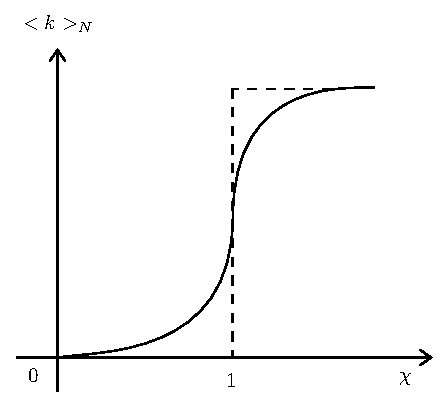
\includegraphics[width=0.4\textwidth]{../lessons/9_image/3.pdf}
\caption{\label{fig:9_3} Thermodynamic average number of open links in a single-ended zipper of \(N\) links.}
\end{figure}

 In order to analyze what happens near 1, we expand \( \chi \equiv 1+\varepsilon  \):

\begin{equation}
\begin{split}
  \log{Z_N} (\chi)  &=  \log{\qty[\frac{1-(1+\varepsilon )^N}{1-(1+\varepsilon )}] }  \\
  & =   \log{\qty[\frac{1-(1+\varepsilon N  + \frac{N(N-1)}{2!}\varepsilon ^2 + \frac{N(N-1)(N-2)}{3!}\varepsilon ^3 +O(\varepsilon ^4))}{\varepsilon }] } \\
  & = \log{\qty[N + \frac{N(N-1)}{2}\varepsilon + \frac{N(N-1)(N-2)}{6}\varepsilon^2 + \dots]  } \\
  & = \log{N} + \log{\qty[1+\frac{N-1}{2}\varepsilon +\frac{(N-1)(N-2)}{6}\varepsilon ^2] } \\
  & = \log{N} + \log{\qty[1+ \frac{N \varepsilon }{2}+ \frac{N^2 \varepsilon ^2}{6}+ \dots] }  \\
  & = \log{N} + \qty( \frac{N \varepsilon }{2} + \frac{N^2 \varepsilon ^2}{6} + \dots) + \frac{1}{2} \qty(\frac{N \varepsilon }{2} + \frac{N^2 \varepsilon ^2}{6} + \dots)^2  + \dots  \\
  & = \log{N}+ \frac{N \varepsilon }{2} + \frac{N^2 \varepsilon ^2}{24} + \dots
\end{split}
\end{equation}
By doing the same for \(   \expval{k}_N = \frac{N \chi^N}{\chi^N-1} - \frac{\chi}{\chi-1} \), one gets
\begin{equation}
  \expval{k}_N = \frac{N}{2} \qty( 1 + \frac{N \varepsilon }{6} - \frac{N^3 \varepsilon ^3}{360} + \dots)
\end{equation}
this is true for \( N \gg 1, \varepsilon \ll 1 \).

At the transition point \( \chi _c =1 \), where \( \varepsilon =0 \):
\begin{equation*}
  \expval{k}_N \simeq \frac{N}{2}
\end{equation*}
We can define the variation (slope per site) as a response function (the derivative with respect to the parameter):
\begin{equation}
  \frac{1}{N}\dv{\expval{k} }{\varepsilon } \simeq \frac{N}{12} - \frac{N^3 \varepsilon ^3}{240} + \dots
\end{equation}
It is max at \( \varepsilon =0 \) and diverges as \( N \rightarrow \infty  \) (linearly). The response function diverges linearly to \emph{N}. This is a good signal that we have a transition.
The temperature \( T_c \) corresponding to the pole \( \chi=1 \) is given
  \begin{equation}
    G e^{-\varepsilon _0 /k_B T_C}  = 1
  \end{equation}
Hence
\begin{equation}
  T_C = \frac{\varepsilon _0}{k_B \log{G} }
\end{equation}
Note that as \( G \rightarrow 1 \), \( T_c \rightarrow 0 \). For \( G=1 \) there is no solution and hence the model does not display a phase transition for any finite \emph{T}! This is telling you that if \( G=1 \) what is important it is the energy, you have no entropy as disorder. At that point everything can happen.
\begin{remark}
Despite the model is \( 1D \), for \( G>1 \) there is a phase transition. This is due to two contributions:
\begin{enumerate}
\item Existence of forbidden configuration (infinite energy). Necessary condition for a phase transition in \( d=1 \) with finite range interactions.
\item Degeneracy of the excited state (\emph{G}).
\end{enumerate}
\end{remark}

\subsection{Transfer matrix method for the Kittel model}
The idea is: we want to map this model to an Ising model. The spin like model consists on associating to each bond a spin such that \( S_i = 0 \) if the \emph{i}-esim bond is \emph{closed} , while \( S_i = 1, \dots, G \) if the \emph{i}-esim bond is \emph{open} with \emph{G} possible orientations.
\begin{itemize}
  \item Case: \( S_i \neq 0 \) open. We have two subcases:
  \begin{itemize}
  \item \( S_{i-1}\) open: \( S_{i-1} \neq 0 \Rightarrow E (S_i \neq 0 | S_{i-1} \neq 0) = \varepsilon _0\).
  \item \( S_{i-1}\) closed: \( S_{i-1} = 0 \Rightarrow  E (S_i \neq 0 | S_{i-1} = 0) = \varepsilon _0 + V_0 \)
  \end{itemize}
\item Case: \( S_i = 0 \) closed. We have \( E (S_i=0)=0 \) irrespective of \( S_{i-1} \).
\end{itemize}
Therefore
\begin{equation}
  E ( S_i, S_{i-1}) = ( \varepsilon _0 + V_0 \delta _{S_{i-1},0}) (1- \delta _{S_i,0})
\end{equation}
The boundary condition is \( S_N =0 \) (always closed).
The full Hamiltonian of the model can be written as (it could be also a function of delta, but it is not a problem):
\begin{equation}
  \mathcal{H}_N = \varepsilon _0 (1- \delta _{S_1,0}) + \sum_{i=2}^{N-1} (\varepsilon _0 + V_0 \delta _{S_{i-1},0})(1- \delta _{S_i,0})
\end{equation}
THe Kittel's version is obtained by assuming \( V_0 = \infty  \).

The partition function is
\begin{equation}
  Z_N = \sum_{\{ S \}  }^{} \exp (-\beta \mathcal{H}_N)
\end{equation}
In order to implement the transfer matrix formalism we rewrite \( Z_N \) as follows (DUBBIIOOOOOO per la prossima equation )
\begin{equation}
  Z_N = \sum_{\{ S \}  }^{} e^{-\beta \varepsilon _0 (1- \delta _{S_1,0})}  \prod_{i=1}^{N-2} e^{-\beta \varepsilon _0 (1- \delta _{S_{i+1},0}) \qty(\dots) \qty(1 + (e^{-\beta V_0}-1 ) \delta _{S_i,0}(1- \delta _{S_{i+1},0}))  }
\end{equation}
Consider the Kittel model, \( V_0 = \infty  \) which implies \( \exp (-\beta V_0) = 0  \). We can define the transfer matrix as
\begin{equation}
  \mathbb{T} = \{ \bra{S} \mathbb{T} \ket{S'} \equiv t_{S,S'}   \}
\end{equation}
where
\begin{equation}
t_{S,S'} = e^{-\beta \varepsilon _0 (1- \delta _{S',0})} [1 - \delta _{S,0} (1- \delta _{S',0})]
\end{equation}
or in matrix form
\begin{equation}
  \mathbb{T} =
  \begin{bmatrix}
    1 & 0 & \dots \dots 0 \\
    1 & a & \dots \dots a \\
    \vdots & \vdots   & \vdots \\
        \vdots & \vdots &  \vdots \\
        1 & a & \dots \dots  a
  \end{bmatrix}
\end{equation}
where \( a \equiv e^{-\beta \varepsilon _0}  \).

The first think to notice that the constraint that the bond \( S_{i+1} \) cannot be open if bond \( S_i \) is closed (\( S_i =0 \) ) yields the null entries in the first row of \( \mathbb{T} \). This violates the hypothesis of the Perron-Frobenius theorem!

The matrix \( \mathbb{T} \) has three differen eigenvalues
\begin{equation}
  \lambda _1 = Ga, \quad \lambda _2 =1, \quad \lambda _1 = 0
\end{equation}
The partition function can be written as
\begin{equation}
  Z_N = (1,a, \dots,a) \mathbb{T}^{N-2} \begin{pmatrix}
  1 \\
  1 \\
  \vdots \\
  1
  \end{pmatrix}
\end{equation}

\begin{equation}
  \lambda _1 \rightarrow \va{v}_1 = \begin{pmatrix}
  0 \\
  1 \\
  \vdots \\
  1
  \end{pmatrix},
  \qquad
  \lambda _2 \rightarrow \va{v}_2 = \begin{pmatrix}
  1-Ga \\
  1 \\
  \vdots \\
  1
  \end{pmatrix}
\end{equation}
We can then write
\begin{subequations}
\begin{align}
  \begin{pmatrix}
  1 \\
  a \\
  \vdots \\
  a
\end{pmatrix}  &= \frac{a(1-Ga)-1}{1-Ga} \va{v}_1 + \frac{1}{1-Ga}\va{v}_2 \\
\begin{pmatrix}
1 \\
1 \\
\vdots \\
1
\end{pmatrix}  &= \frac{-Ga}{1-Ga} \va{v}_1 + \frac{1}{1-Ga}\va{v}_2
\end{align}
\end{subequations}
Therefore
\begin{equation}
  Z_N = \frac{1-(Ga)^N}{1-Ga} = \frac{1-(G e^{-\beta \varepsilon _0} )^N}{1-G e^{-\beta \varepsilon _0} }
\end{equation}
or
\begin{equation}
  Z_N = \frac{1}{1-G e^{-\beta \varepsilon _0} } (-\lambda _1^N + \lambda _2^N)
\end{equation}
Since in the thermodynamic limit only the contribution of the largest eigenvalue matters for \( f_b \) we have
\begin{equation}
  f_b = - k_B T \ln{\text{max} (\lambda _1, \lambda _2)}
\end{equation}
\begin{remark}
Given that the \( \lambda _1 \) and \( \lambda _2 \) are positive, analytic function of \emph{T} (\( \lambda _1 = Ga, \lambda _2=1 \) ). In order to have a phase transition
(i.e. non analiticity of \( f_b \)) the two eigenvalues must cross for a given value of \emph{T}. It is true if and only if:
\begin{equation}
  G a_c =1 \Leftrightarrow G e^{-\beta _c \varepsilon _0} = 1  \Leftrightarrow T_c = \frac{\varepsilon _0}{k_B \ln{G} }
\end{equation}
It is agree with previous calculation.
\end{remark}


\section{Transfer matrix for \( 2D \) Ising}
The bibliography of this section is  \cite{9_lesson_1},\cite{9_lesson_2},\cite{9_lesson_3}.

Dimensional reducation from \emph{d} to \emph{d-1}. You can to the same for the 3D Ising model. In order to go smoothly to the one dimensional to the two dimensional the idea is to solve the Ising model to surfaces.

Consider a square lattice with \emph{N} rows and \emph{M} colums, as in Figure \ref{fig:9_4}, with periodic boundary conditions (wrapped around a torus).
The spin in a site is identifed by \( S_{\text{site}} = S_{m,n} \).
\begin{figure}[h!]
\centering
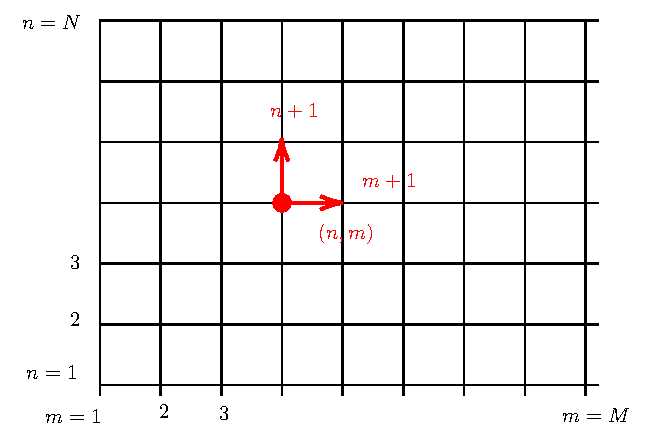
\includegraphics[width=0.6\textwidth]{../lessons/9_image/4.pdf}
\caption{\label{fig:9_4} Description.}
\end{figure}
The Hamiltonian is (if \( H \neq 0 \) we have also the term with the \emph{h}):
\begin{equation}
\begin{split}
  -\beta \mathcal{H}_ \Omega  ( \{ S \}  ) &= k \sum_{\expval{ij} }^{} S_i S_j + h \sum_{i}^{} S_i  \\
  & = k \sum_{n=1}^{N} \sum_{m=1}^{M} (S_{m,n} S_{m+1,n}+S_{m,n}S_{m,n+1}) + h \sum_{n=1}^{N} \sum_{m=1}^{M} S_{m,n}
\end{split}
\end{equation}
in fact
\begin{equation}
  \sum_{\expval{i,j} }^{}  \rightarrow \sum_{i,j \in nn(i)}^{} \quad \Rightarrow   S_{m,n} \rightarrow S_{m+1,n}
\end{equation}

The Hamiltonian can be rewritten as follows:
\begin{equation}
  -\beta \mathcal{H}_ \Omega  ( \{ S \}  ) = \sum_{m=1}^{M} \qty[E[\mu _m, \mu _{m+1}] + E[\mu _m]]
\end{equation}
where the first term is the interaction between columns (two body interaction), the second term is the one body interaction of one column. Moreover, the \( \mu  \)  is a \emph{m} dimensional vector, in particular each \( \mu _m \) represents the set of \emph{N} spins along column \emph{m}:
\begin{equation}
  \mu _m = \{ S_{m,1}, S_{m,2}, \dots, S_{m,N} \}
  \label{eq:9_1}
\end{equation}
We have:
\begin{subequations}
\begin{align}
E [ \mu _m,h] &= k \sum_{n=1}^{N} S_{m,n} S_{m,n+1} + h \sum_{n=1}^{N} S_{m,n} \\
  E [\mu _m, \mu _{m+1},h] & = k \sum_{n=1}^{N} S_{m,n} S_{m+1,n}
\end{align}
\end{subequations}
where the first equation is the one body interaction, while the second equation represents the interaction between neirest neighbours columns.

We can write a transfer matrix between these new variables. The transfer matrix permit to transfer along the \emph{m}. To make it simpler suppoe \( h=0 \) (so the energy does not depend on h):
\begin{equation}
  \bra{\mu _m} \mathbb{T} \ket{\mu _{m+1}} = \exp [ k(E [\mu _m, \mu _{m+1}] + E [ \mu _m])]
  \label{eq:9_2}
\end{equation}
Now we have to diagonalize. In the 2x2 tranfer matrix in the two dimensional we have 2 possible values. Now we have to do the same in principle, but we have to do for all of the \eqref{eq:9_1}.
\( \mathbb{T} \) is a matrix of dimension \( 2^N \times 2^N \). In the thermodynamic limit is an infinite matrix (violation of Perron-Frobenius). According to the formalism
\begin{equation}
  Z_{N} (k,h) = \Tr(\mathbb{T}^N)
\end{equation}
To find the eigenvalues of \( \mathbb{T} \) given by  \eqref{eq:9_2} is highly non trivial. The big problem it is that in the thermodynamic limit is that the dimension of the transfer matrix goes to infinity, then it is diffucult to be diagonalized. This was first achived by Onsanger in 1944 for the case \( H=0 \) and in the \( N \rightarrow \infty  \) limit. The result is given by
\begin{equation}
  f_b (T) = -k_B T \log{\qty(2 \cosh(2 \beta J))- \frac{k_B T}{2 \pi} \int_{0}^{2\pi} \log{\qty[\frac{1}{2}\qty(1+ \sqrt{1-g^2 \sin^2(\Phi) } )] } \dd[]{\Phi }  }
\end{equation}
that is the density bulk free energy, where
\begin{equation}
  g = \frac{2}{\cosh(2 \beta J)\coth(2 \beta J)}
\end{equation}
The equation for the critical \emph{T} is
\begin{equation}
  2 \tanh^2 \qty(\frac{2J}{k_B T_c}) = 1 \quad \Rightarrow T_c \simeq 2,264 J/k_B \neq 0!
\end{equation}
One can also show that
\begin{equation}
  c \propto A \qty[-\ln{\qty(1- \frac{T}{T_c}) } + B  ]
\end{equation}
The specifi heat displays at the transition a logarithmic divergence (no power law!). Therefore the in \( d=2 \)  the Ising model as \( \alpha _{\text{\tiny Ising 2D}} =0\).
You do Montecarlo simulation.















\end{document}
